\section{Results}
In this section we present results of runing the simulation described in the previous section. The subsections below focus on the following research questions, 

\begin{itemize}
  \item How well does the RFEA derived ion energy distribution function represents the actual energy distribution function of ions at the bounding electrode (i.e., at G$_0$)? 
  \item What is the effect of ion space charge inside the RFEA on the space potential and electric field?  
  \item What is the effect of different spacings between grids on the RFEA derived ion energy distribution function when compared to the actual one at the bounding electrode?
  \item How does the pressure transparency of the RFEA changes with pressure? For any given pressure, does the pressure transparency change with the discrimination, G$_2$, voltage? 
\end{itemize}


\subsection{Ion energy distribution profile}
Fisrt, we run the simulation at various pressures and compared the derived ion energy disribution function with the actual energy distribution as recorded in the model at G$_0$. The RFEA configuration is as follows: 2332 stack, G$_1$=C=-60~V, G$_3$=-70~V, grid transparency 100~\%. The plasma sheath potential used is AC with maximum voltage difference across the sheath of 2000~V (i.e., V$_\text{pk-pk}$), the radio-frequency 13.56~MHz, and the plasma density $10^{16}$~m$^{-3}$. The pressure settings are 0.5, 1.0, 2.0, 5.0, 7.5 and 10.0~Pa. The model is run sweeping grid G$_2$ voltage setting from 0 to 1500~V in steps of 25~V. The number of ions whose trajectory is simulated per G$_2$ voltage step is 25000. The starting time for each ion is randomized uniformly across the radio-frequency period to represent that ions may enter the sheath at any point during the RF cycle. Each ion trajectory is followed for a total time of 1~$\mu$s. 

Figure~\ref{fig:IVcurve} shows the characteristic current-voltage curve for each model RFEA scan. The vertical axis is the ion count at the collector position. The ion count drops as the pressure is increased. 

\begin{figure}[htbp]
\centering
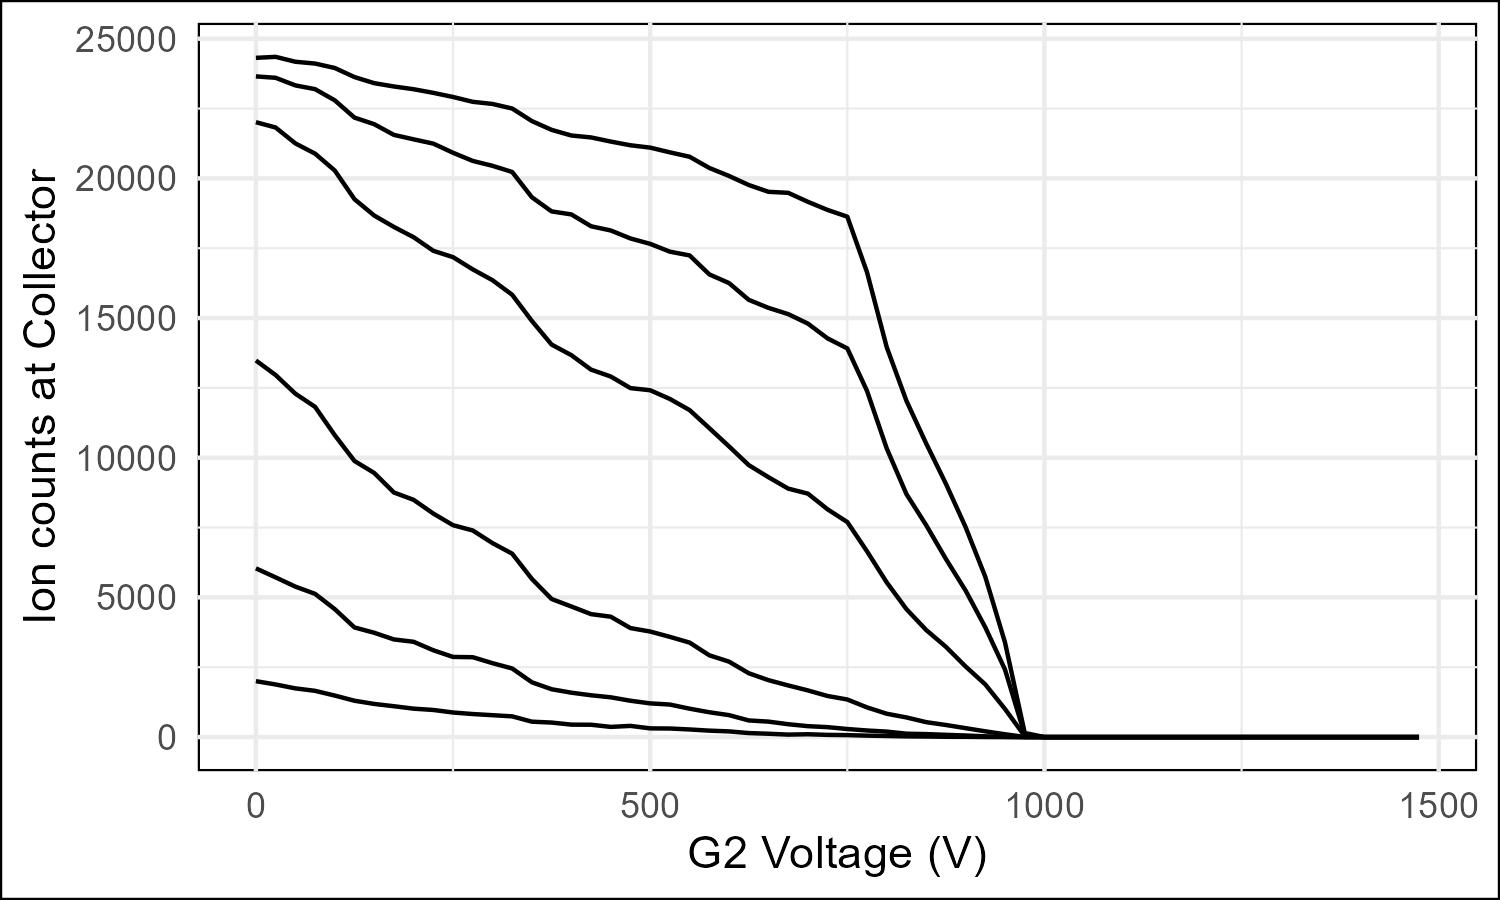
\includegraphics[width=0.45\textwidth]{Figures/IVcurve.jpeg}
\caption{Current-voltage characteristic curves where the current is represented by the ion count collected at the collector position. The curves from highest ion count value to lowest correspond to pressure settings from 0.5 to 10.0~Pa.}
\label{fig:IVcurve}
\end{figure}

The first derivative of the ion current is proportional to the ion energy distribution function~\cite{Hutchinson1987}. The set of curves on the left of Figure~\ref{fig:PressureScan} shows the first derivative of the curves in Figure~\ref{fig:IVcurve}. The derivatives are normalized and plotted with an offset in the vertical axis from lowest pressure setting at the top to highest pressure setting at the bottom. The ion energy distributions derived from the ion counts at the collector in the simulated RFEA for the various pressure settings can be contrasted with the actual ion energy distributions recorded at G$_0$, before the ions transport through the RFEA. These IEDFs are shown on the right of Figure~\ref{fig:PressureScan}. These scan was repeated using a smaller integration time step for the ion trajectories, $dt=10$~ps, to assess any potential artifact introduced in the simulation by the trajectory integration method, and no substantial qualitative difference on the energy distribution functions was observed (not shown). The derived IEDF at the collector exhibits more noise than the IEDF at G$_0$ due to the nature of the numerical derivative of the collector ion count; i.e., numerical derivatives of any parameter always ampiflies the parameter's noise. Here, a centered finite difference method was used to differentiate the Collector ion counts. All curves are shown without any smoothing. Still, both distributions show similar features, which is expected as ion-neutral collisions can not affect the shape of the ion energy distribution function~\cite{Baloniak2010}.   

\begin{figure}[htbp]
\centering
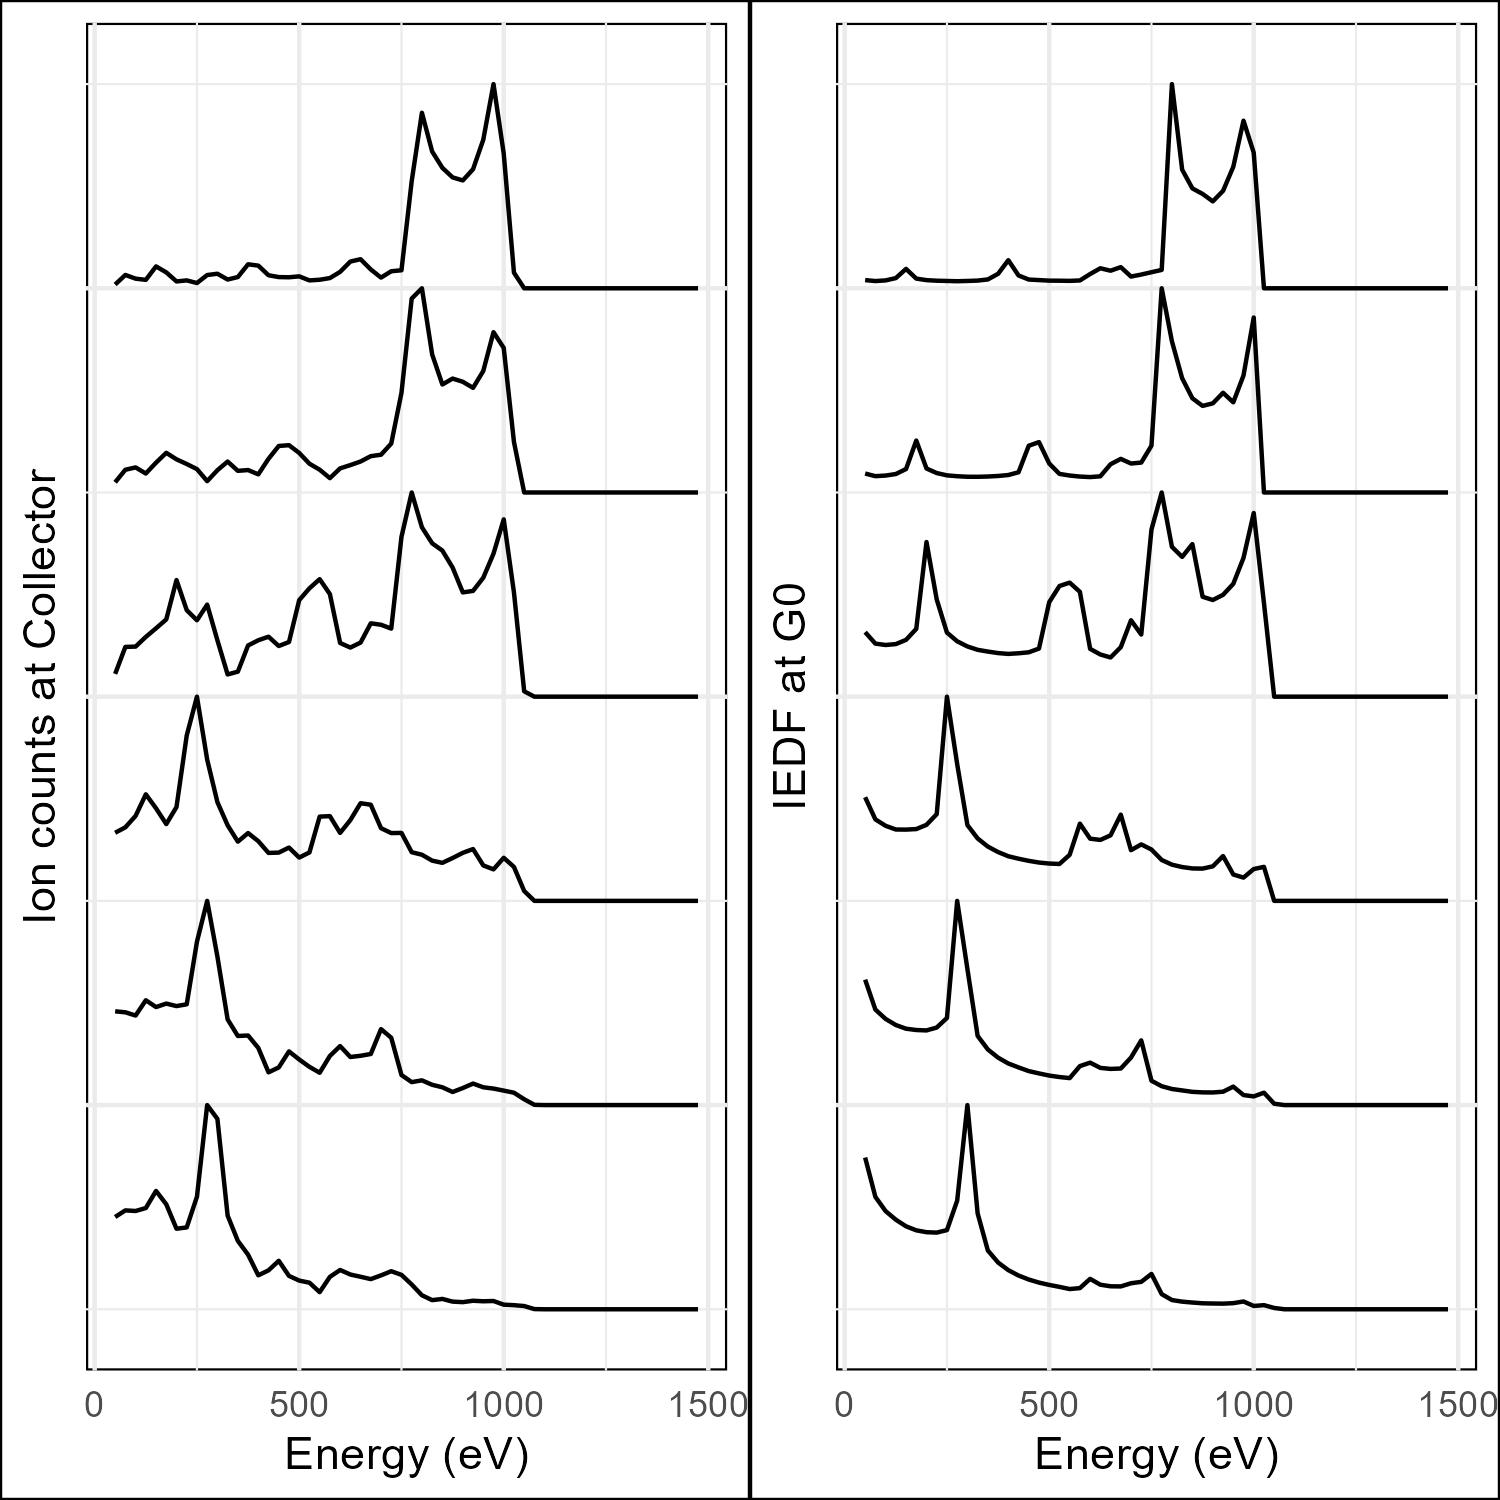
\includegraphics[width=0.45\textwidth]{Figures/PressureScan.jpeg}
\caption{Ion energy distribution functions. Left: First derivative of the current-voltage characteristic curves of Figure~\ref{fig:IVcurve}. Right: Plot of the ion energy distribution as recorded in the simulation at G$_0$, before ion transport through the RFEA. Both set of curves are normalized. The curves from top to bottom correspond to pressure settings from 0.5 to 10.0~Pa.}
\label{fig:PressureScan}
\end{figure}

The ion energy distributions of Figure~\ref{fig:PressureScan} exhibit a series of peaks which are the result of the oscillating plasma sheath and ion collisions with the background gas. More specifically, the sheath modulation, i.e., the time varying sheath edge and sheath electric field, can shape specific features of the IEDFs~\cite{Wild1989,Wild1991}. 




Second, we run the simulation at various radio-frequencies and compared the derived ion energy disribution function with the actual energy distribution as recorded in the model at G$_0$. The RFEA configuration is the same as the previous scan including the sheath potential maximum voltage difference 2000~V (i.e., V$_\text{pk-pk}$), the plasma density $10^{16}$~m$^{-3}$, and fixed pressure setting of 0.5~Pa. The model is run sweeping grid G$_2$ voltage setting from 0 to 1750~V in steps of 25~V. The number of ions whose trajectory is simulated per G$_2$ voltage step is 25000. The starting time for each ion is randomized uniformly across the radio-frequency period and each ion trajectory is followed for a total time of 1~$\mu$s. 

Figure~\ref{fig:IVcurve_FrequencyScan} shows the characteristic current-voltage curve for each model RFEA radio-frequency scan. The vertical axis is the ion count at the collector position. The set of curves on the left of Figure~\ref{fig:FrequencyScan} show the first derivative of the curves in Figure~\ref{fig:IVcurve_FrequencyScan}. The derivatives are normalized and plotted with an offset in the vertical axis from lowest radio-frequency setting at the top to highest at the bottom. The IEDFs recorded at G$_0$ are shown on the right of Figure~\ref{fig:FrequencyScan}. The distribution functions show a wider energy gap (between the lower energy peak to the higher energy peak) as the radio-frequency driving the sheath is reduced~\cite{Lieberman2005}. The lower frequencies have a stronger modulation effect on ions in transit through the sheath. However, there is no shift in the average of the energy peaks (mid point between the two peaks) as reported by Gahan et al.~\cite{Gahan2008}. Moreover, everything else being equal, as the radio-frequency is increased the maximum ion energy is approximately half the maximum voltage across the sheath; i.e., at 27.12~MHz, a 2~kV$_{pk-pk}$ sheath modulation accelerates ions up to approximately 1~keV.  

\begin{figure}[htbp]
\centering
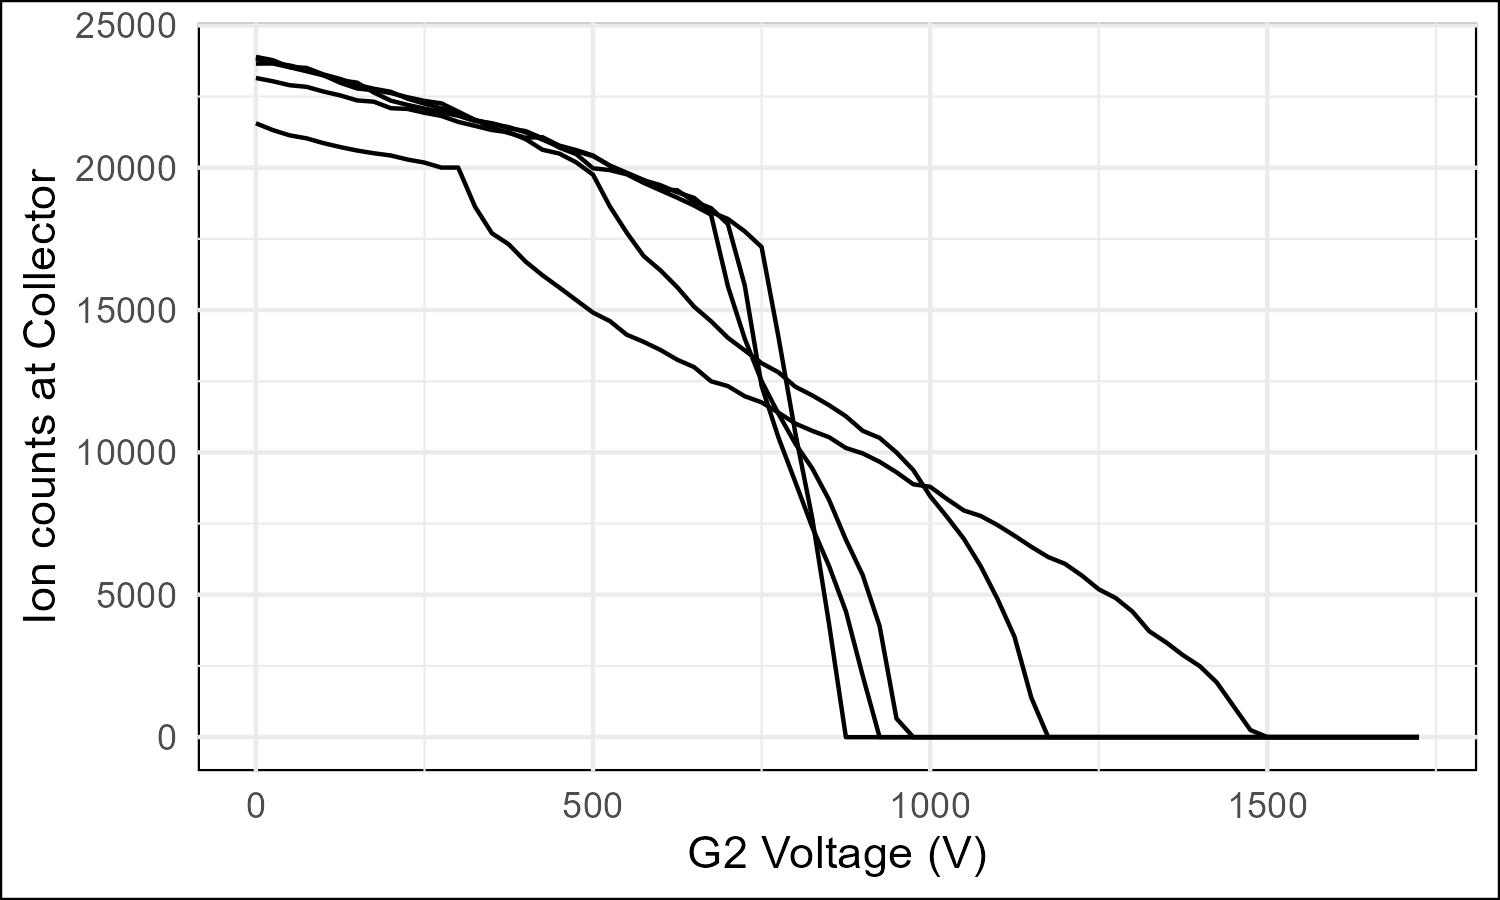
\includegraphics[width=0.45\textwidth]{Figures/IVcurve_FrequencyScan.jpeg}
\caption{Current-voltage characteristic curves where the current is represented by the ion count collected at the collector position. The curves correspond to frequency settings from 2~Mhz to 27.12~MHz. The pressure was set to 0.5~Pa. }
\label{fig:IVcurve_FrequencyScan}
\end{figure}

\begin{figure}[htbp]
\centering
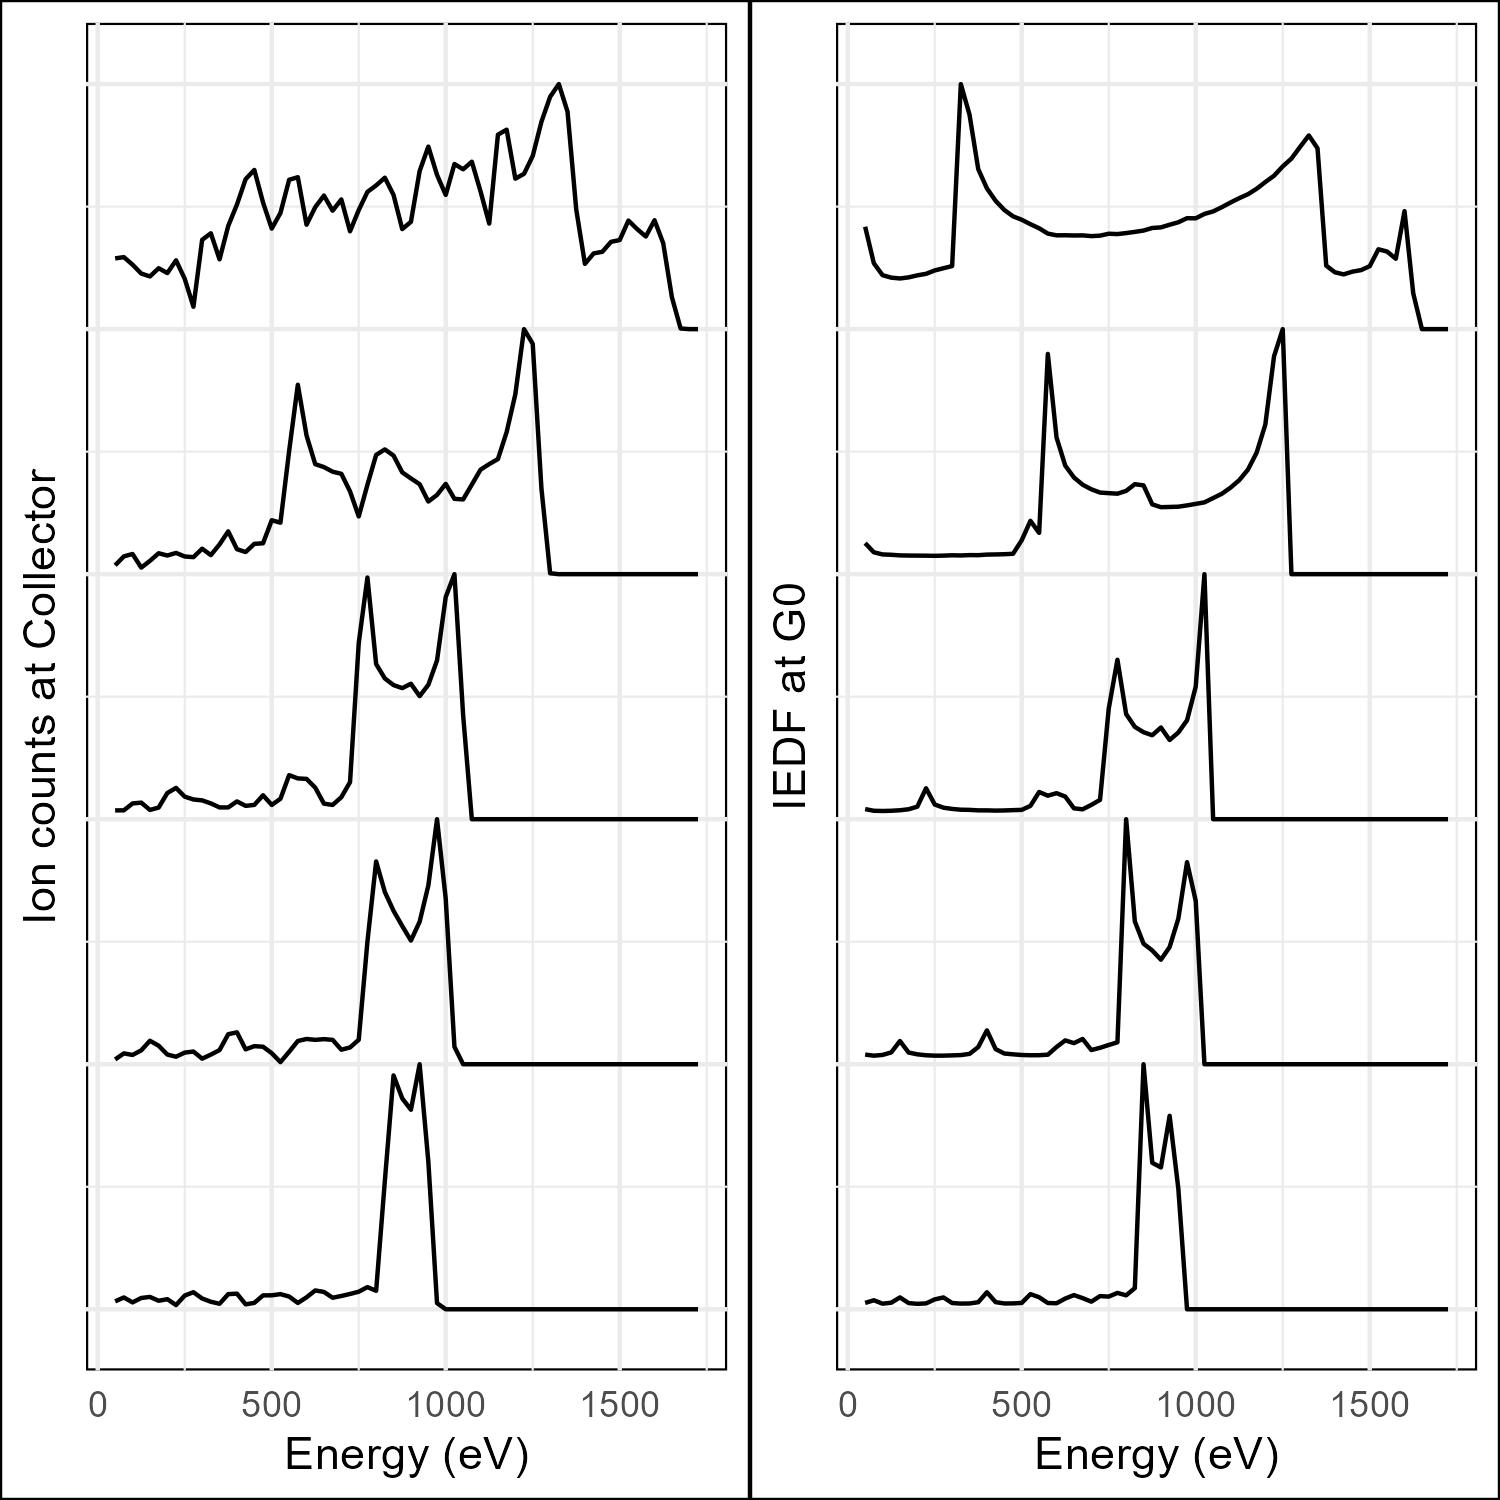
\includegraphics[width=0.45\textwidth]{Figures/FrequencyScan.jpeg}
\caption{Ion energy distribution functions. Left: First derivative of the current-voltage characteristic curves of Figure~\ref{fig:IVcurve}. Right: Plot of the ion energy distribution as recorded in the simulation at G$_0$, before ion transport through the RFEA. Both set of curves are normalized. The curves from top to bottom correspond to frequency settings from 2~MHz to 27.12~MHz. The pressure was set to 0.5~Pa.}
\label{fig:FrequencyScan}
\end{figure}





\subsection{Space charge inside the RFEA}
In high density plasmas, the ion current may be sufficiently high to allow for the build up of space charge within the RFEA~\cite{Hutchinson1987}. The charge build up may be highest for G$_2$ voltages at which most of the ion current is cut off. The model is used by simulating multiple ion trajectories through the plasma sheath and the RFEA. The trajectories are run for a maximum time of 1~$\mu$s. For each trajectory a random number is generated between 0 and 1 and is multiplied by the maximum time. This simulates the condition that not all ions depart the plasma at the same time and allow for spatial charge build up from the plasma sheath. The grid transparency is set to 50~\% to simulate ions collected by the grids and therefore removed from the space charge build up. The final position of the ions for each trajectory, if not collected by a grid or the collector, is recorded and a space charge density can be plotted. This simulation can be repeated for various G$_2$ voltages, pressures, sheath voltage, and radio-frequency.  






\subsection{Pressure transparency estimate}
The ion current to the collector in an RFEA can be attenuated mainly by two factors: a geometrical transparency factor, and a collisional transparency factor.  

First, each grid in the analyzer has a open area which can be used to estimate a geometrical transparency. Typically, the open area is 50~\%. The geometrical transparency is influenced by variations in the dimensions of grids openings, the number of openings in each grid, the alignment between grids and lensing effects due to the electric field distortion around the grid surface. As discussed in the description section, we can assign a geometrical transparency to every grid. The geometrical transparency (P$_g$) is the fraction of ions that may reach the collector where the impediment is only due to geometrical effects.  

Second, even though the spacing between grids is typically small (i.e., in the order of 100s of $\mu$m) ion collisions with neutrals may occur even at low pressures. As described before, the dominant collision process is charge exchange which effectively takes away all the energy gained by the ion in the sheath. Therefore, any collisions before the discriminator G$_2$ or at a distance after the discriminator grid where the space potential is below the potential of the collector would prevent said ion from reaching the collector~\cite{Baloniak2010}. The collisional transparency (P$_c$) is the fraction of ions that may reach the collector where the impediment is only due to ion collisions with the neutral background gas. 

The total ion current attenuation is the product of the two transparency factors.
\begin{equation}
P_{\text{total}} = P_\text{g} + P_\text{c}
\end{equation}

The collisional transparency ($P_c$) can be estimated from a theoretical approach as follows~\cite{Baloniak2010}, 
\begin{equation}
P_c = e^{- L / \lambda_i} 
\end{equation}
Where $L$ is the size of the RFEA stack, and $\lambda_i$ is the ion mean free path. The ion mean free path is
\begin{equation}
\lambda_i = (n_g \sigma)^{-1}
\end{equation}
Where $n_g$ is the density of the neutral background gas (in m$^{-3}$), and $\sigma$ is the collision cross section for ion-neutral collisions (in m$^2$). Note that the collision cross section is a function of the ion energy; see subsection~\ref{IonCollision}. However, for the purpose of a simple approximation the cross section can be taken as a constant value. Such simple approximation is used in the sheath model to make adjustments to account for ion collisions; see equation~\ref{eq:lambda_i}. The gas density can be estimated from the ideal gas law, 
\begin{equation}
n_g = \frac{p}{k_B T_g}
\end{equation}    
Where $p$ is the pressure of the background gas in Pascal, $k_B$ is the Boltzmann constant, and $T_g$ is the temperature of the background gas in Kelvin. Using this expression for the gas density we can estimate the collisional transparency as
\begin{equation}
P_c = e^{- L \sigma p / k_B T_g}
\end{equation}
Alternatively, using equation~\ref{eq:lambda_i}, the collisional transparency can be expressed as
\begin{equation}\label{eq:CollisionalTrasparency}
P_c = e^{- 30 L p / 0.13332237}
\end{equation}
By comparing the last two equations we can determine that if gas temperature is set to 300~K the collisional cross section used in equation~\ref{eq:lambda_i} is $\sigma \approx 93.2 \times 10^{-20}$~m$^2$. However, the cross section data shown in Figure~\ref{fig:CrossSectionsArgon} indicates that such value corresponds to ions with energies well below 1~eV. The choice of cross section value in this approximation of the collisional transparency has a strong influence in the outcome of the calculation.  

The pressure scan results can be used to estimate the collisional transparency. Using a similar procedure as that done experimentally, we can compare the number of ions reaching C with those passing through G$_0$ with no ion discrimination, i.e., G$_2 =0$. In the simulation, for each G$_2$ voltage setting 25000 ion trajectories were simulated. Therefore, the number of ions reaching the collector when G$_2$ is set to null divided by the 25000 is the collisional transparency. Figure~\ref{fig:CollisionalTransparency} shows the estimated collisional transparency from the pressure scan data between 0.5 and 10~Pa. The graph shows data from scans with a 2332 and 2772 button stack. The theoretical collisional transparency of equation~\ref{eq:CollisionalTrasparency} strongly underestimates the value. Using a collision cross section value of $\sigma \approx 22.5 \times 10^{-20}$~m$^2$ results in better agreement. But would be best to do a fit! That cross section value corresponds to ions with energies around 1~keV which is the upper limit energy for the ions in these simulation for the lowest pressures. As the pressure is increased the mean energies are lower. But as the pressure increases this lower value of cross section results in higher collisional transparencies. which underestimates the effect of collisions reported in the model. This discrepancy suggests that the effect of collisions is therefore more complex than the theoretical formulation.  

The data shown in Figure~\ref{fig:CollisionalTransparency} is fitted to an exponential decay model. The fitted curves, with R$^2 > 0.99$, are
\begin{eqnarray}
P_\text{c:2332} (p) &=& e^{-0.0666 p} \\
P_\text{c:2772} (p) &=& e^{-0.105 p} 
\end{eqnarray}    

\begin{figure}[htbp]
\centering
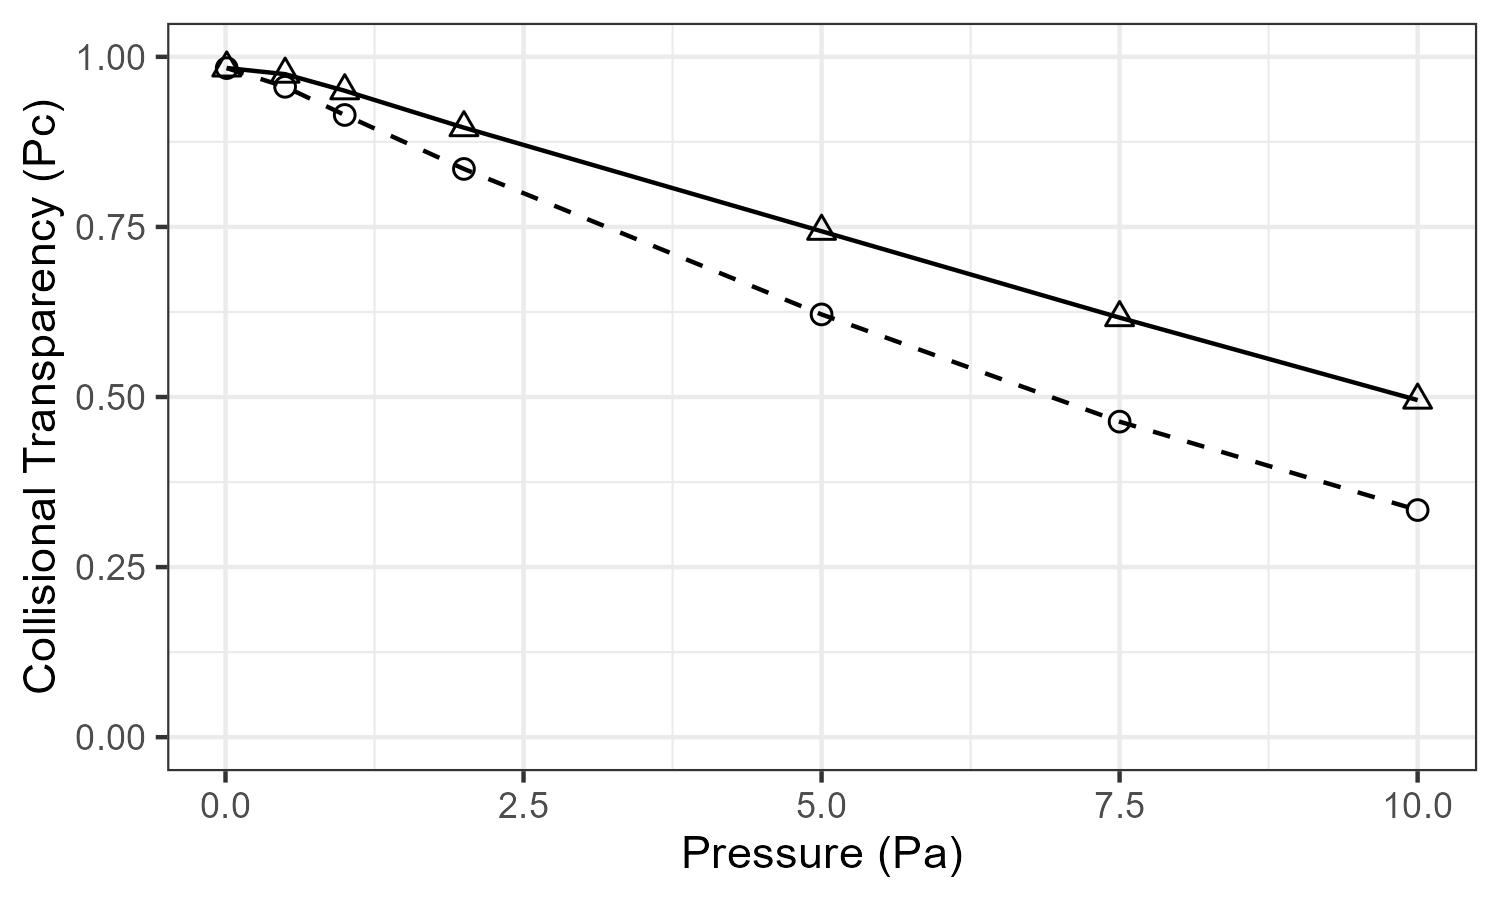
\includegraphics[width=0.45\textwidth]{Figures/CollisionalTransparency.jpeg}
\caption{Estimated collisional transparency (P$_g$) as a function of argon neutral gas pressure. The RFEA button stack configurations are: 2332:triangles, and 2772:cicles. The data is tabulated in Table~\ref{table:CollisionalTransparency}.}
\label{fig:CollisionalTransparency}
\end{figure}


\begin{table}
\centering
\caption{Collisional transparency as a function of pressure from simulations with RFEA button stacks 2332 and 2772. Data is plotted in Figure~\ref{fig:CollisionalTransparency}.}
\label{table:CollisionalTransparency}
\begin{tabular}{rrr}
  \hline
              & Collisional & Transparency \\
Pressure (Pa) & 2332 & 2772 \\ 
  \hline
0.01 & 0.98 & 0.98 \\ 
  0.50 & 0.97 & 0.96 \\ 
  1.00 & 0.95 & 0.91 \\ 
  2.00 & 0.90 & 0.84 \\ 
  5.00 & 0.74 & 0.62 \\ 
  7.50 & 0.62 & 0.46 \\ 
  10.00 & 0.50 & 0.33 \\ 
   \hline
\end{tabular}
\end{table}


Furthermore, a scan at very low pressure, i.e. 0.01~Pa, can be used to get $P_c \approx 1$. The ion counts at the collector for every voltage value of the discriminator G$_2$ at this low pressure can be used as the reference collisional transparency. In this way we evaluate if the collisional transparency varies with G$_2$ voltage. No, this is not possible, as for every G$_2$ voltage the ion current to the RFEA is not the same at different pressures as collisions change the ion energy distribution function. Only at G$_2$ we can compare the ion collection at C. The pressure scan for the 2332 and 2772 stacks are extended to include 0.01~Pa and 0~Pa pressure settings. In the case of the latter, the collisionless sheath model is used. However, the collisionless sheath model estimates a smaller sheath than the collisional at low pressure. This results in discrepancies in the IEDFs at low pressures. The effect of a smaller sheath is that the ion energy peaks appear to be separated a wider distance than when the sheath is larger, as in the case of 0.01~Pa. Figure~\ref{fig:IVcurves2332} and Figure~\ref{fig:IVcurves2772} show the IV curves for the two different button stacks at pressures, 0, 0.01, 0.5, 1, 2, 5, 7.5 and 10~Pa. Figure~\ref{fig:PressureScan2332} and Figure~\ref{fig:PressureScan2772} show the IEDF curves for the two different button stacks at pressures, 0, 0.01, 0.5, 1, 2, 5, 7.5 and 10~Pa. The energy separation in the IEDF peaks is estimated~\cite{Gahan2008} as 
\begin{equation}
\Delta E = \frac{2 e V_0}{ \pi } \frac{ \tau_\text{rf} }{ \tau_\text{i} }
\end{equation} 
Where $V_0$ is the peak to peak radio-frequency modulation voltage across the sheath, $\tau_\text{rf}$ is the radio-frequency period, and $\tau_\text{i}$ is the ion transit time across the sheath. Naturally, a smaller sheath translates to a shorter ion transit time and therefore a larger energy difference $\Delta E$. In other words, the larger the sheath, the longer the ion transit time, and therefore the smaller the peak energy difference. In the collisional model, the lower the pressure, the larger the sheath and therefore the longer the ion transit time and the smaller the peak ion energy difference.  

\begin{figure}[htbp]
\centering
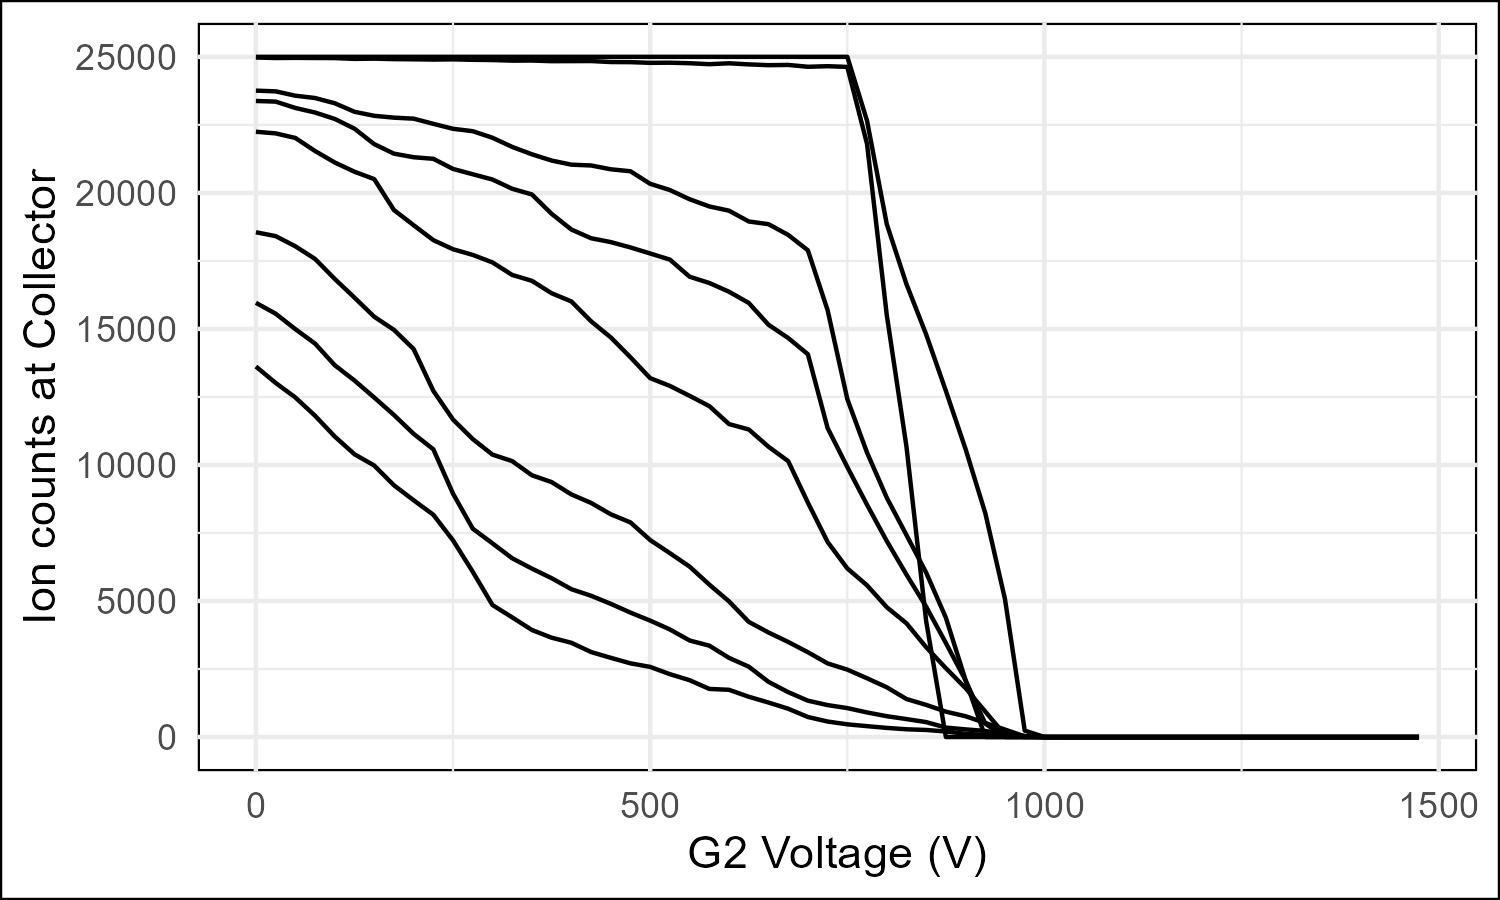
\includegraphics[width=0.45\textwidth]{Figures/IVcurve2332.jpeg}
\caption{IV curves, pressure scan, stack 2332.}
\label{fig:IVcurves2332}
\end{figure}

\begin{figure}[htbp]
\centering
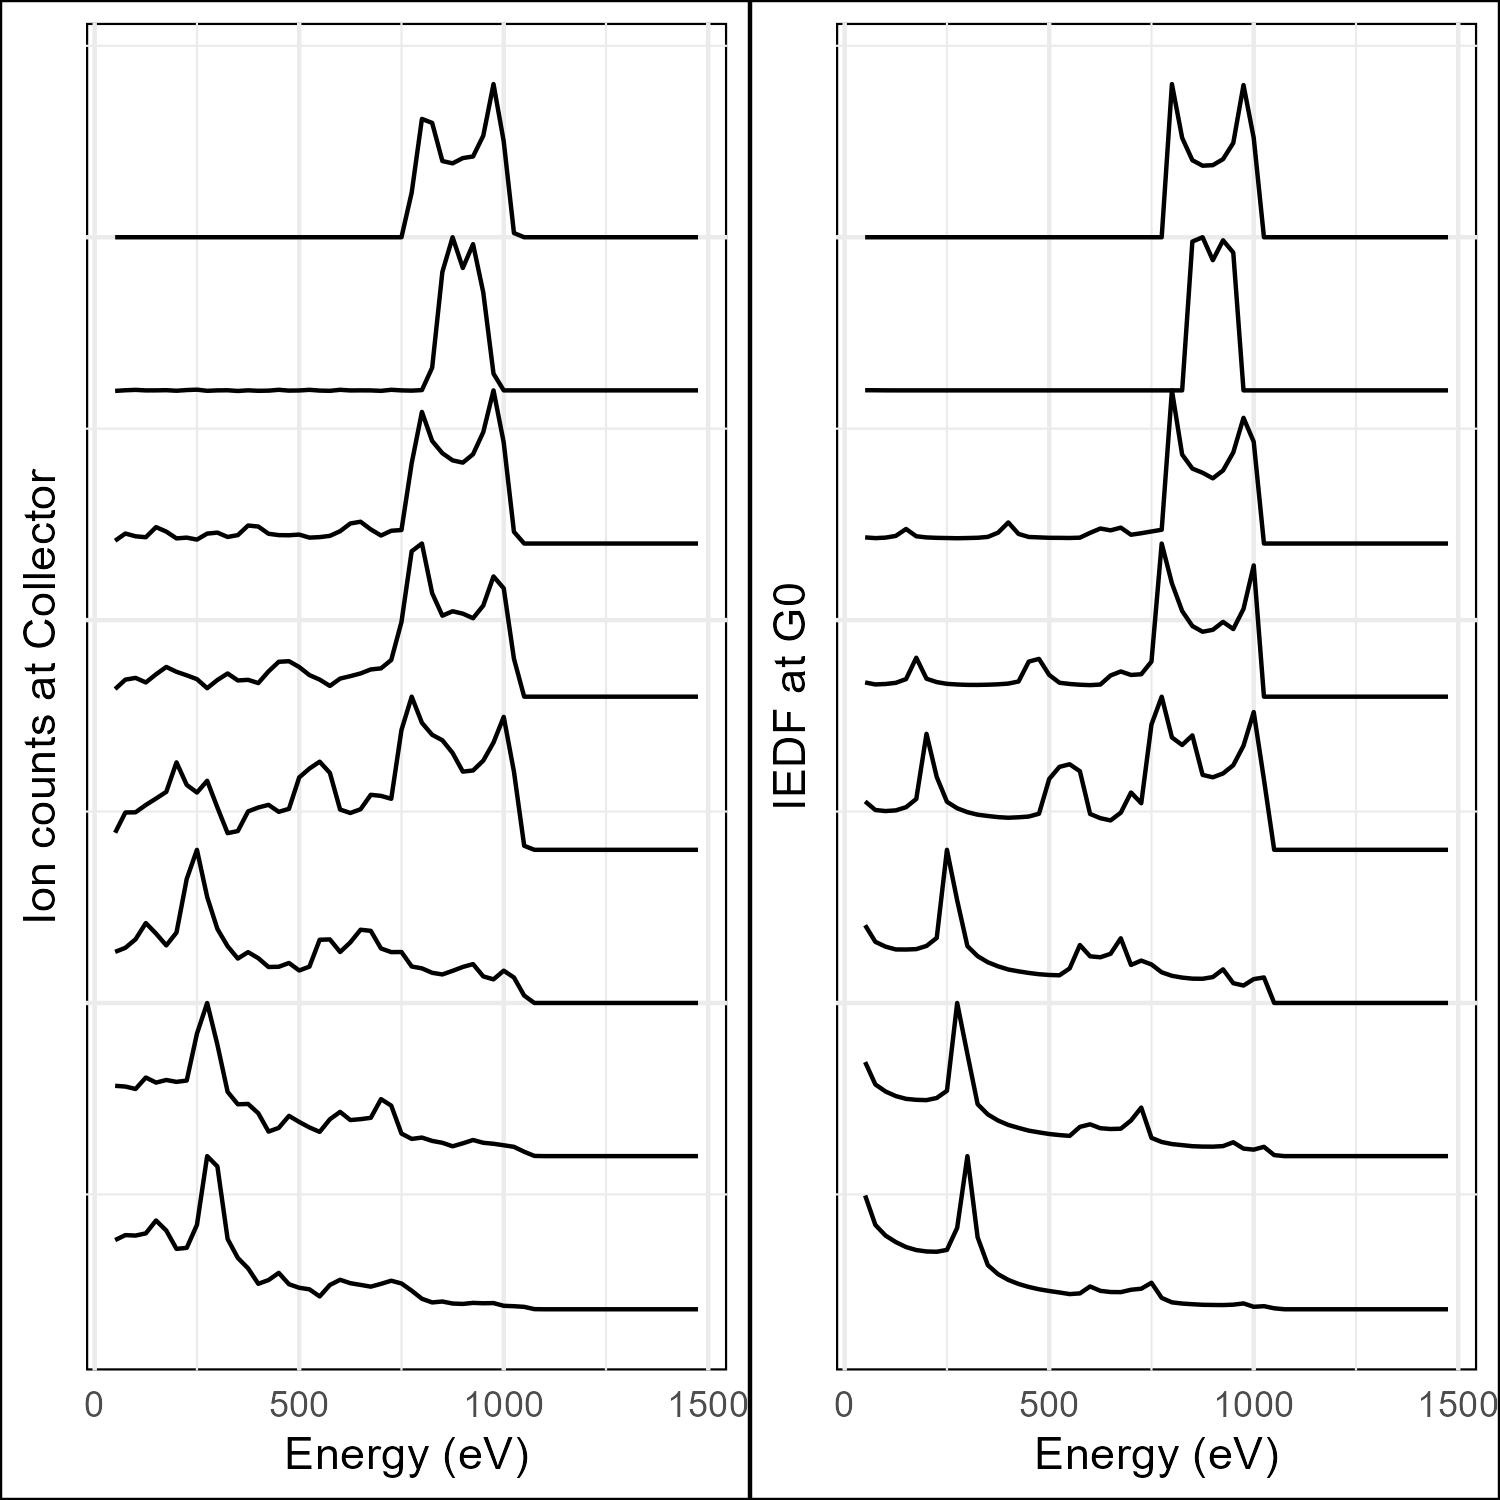
\includegraphics[width=0.45\textwidth]{Figures/PressureScan2332.jpeg}
\caption{IEDF curves, pressure scan, stack 2332.}
\label{fig:PressureScan2332}
\end{figure}

\begin{figure}[htbp]
\centering
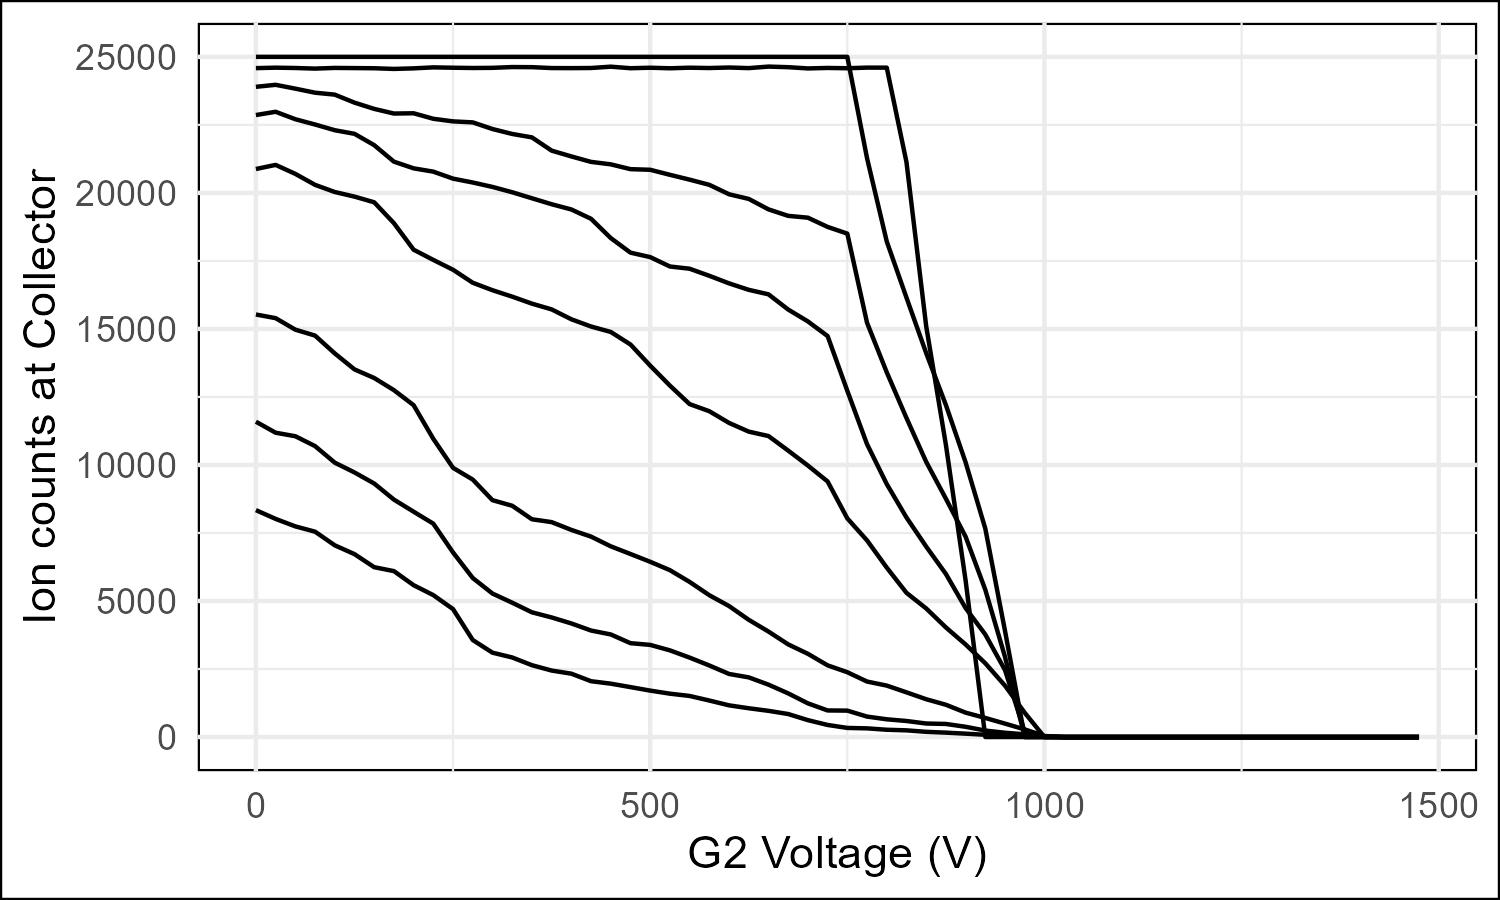
\includegraphics[width=0.45\textwidth]{Figures/IVcurve2772.jpeg}
\caption{IV curves, pressure scan, stack 2772.}
\label{fig:IVcurves2772}
\end{figure}

\begin{figure}[htbp]
\centering
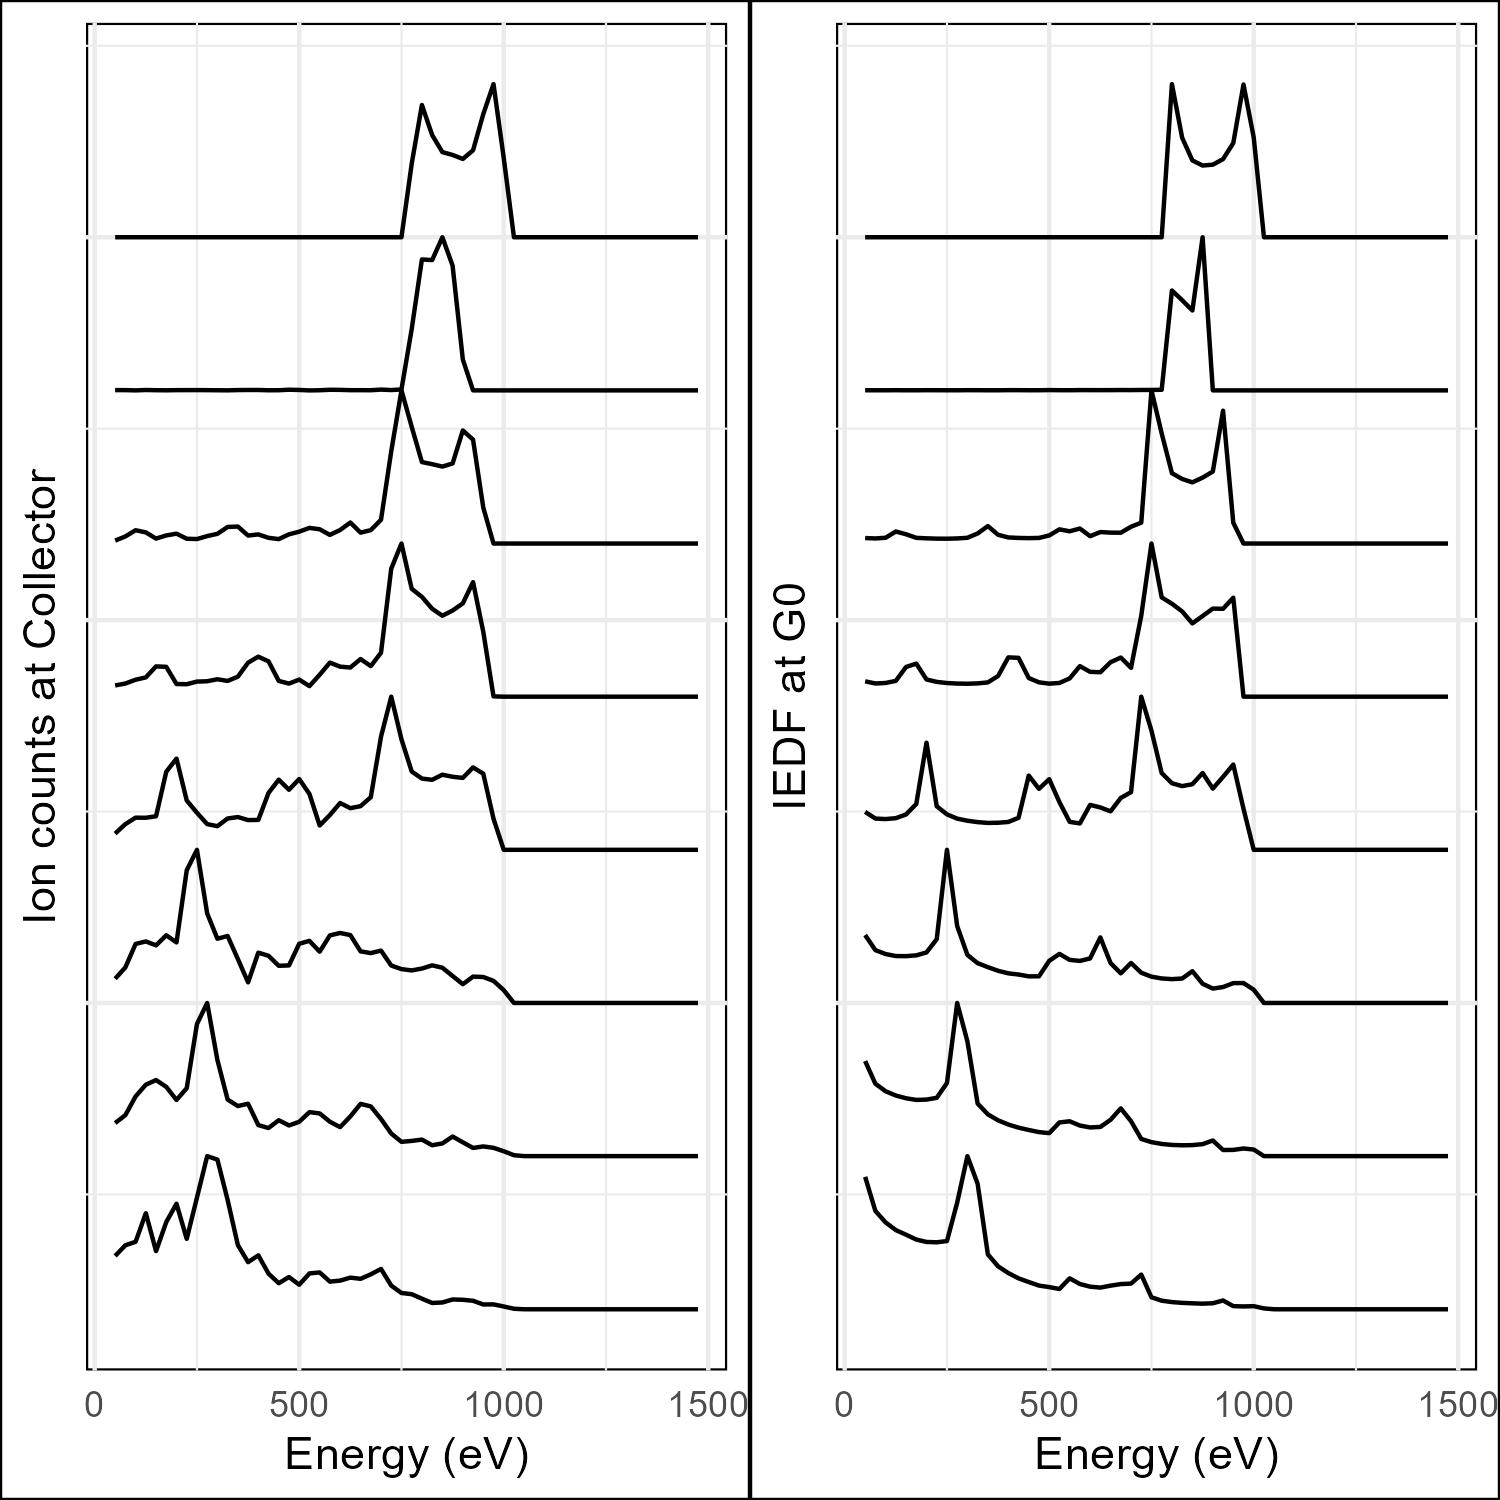
\includegraphics[width=0.45\textwidth]{Figures/PressureScan2772.jpeg}
\caption{IEDF curves, pressure scan, stack 2772.}
\label{fig:PressureScan2772}
\end{figure}
